\documentclass[11pt,a4paper]{article}
\usepackage[margin=2.3cm]{geometry}
\usepackage[T1]{fontenc}
\usepackage[utf8]{inputenc}
\usepackage{lmodern}
\usepackage{amsmath,amssymb}
\usepackage{graphicx}
\usepackage{booktabs}
\usepackage{multirow}
\usepackage{siunitx}
\usepackage{algorithm}
\usepackage{algpseudocode}
\usepackage[numbers,sort&compress]{natbib}
\usepackage{xcolor}
\usepackage[colorlinks=true,linkcolor=blue!50!black,citecolor=blue!50!black,urlcolor=blue!50!black]{hyperref}
\usepackage{caption}
\captionsetup{font=small,labelfont=bf}
\sisetup{group-separator={,},group-minimum-digits=4}

\newcommand{\CL}{C_{\mathrm{L}}}
\newcommand{\CG}{C_{\mathrm{G}}}
\newcommand{\pfail}{p_{\mathrm{fail}}}

\title{When Does Local Path Repair Pay Off?\\[2pt]
\large A Break-Even Analysis of Local Repair versus Global and Incremental Replanning\\
for Mobile Robots with a Limited Perception Range}

% Further author(s) / supervisor to be added after confirmation.
\author{Akram Ahmed Ahmed Abdullah\thanks{[Department, University, City, Country]. Corresponding author: [e-mail].}}

\date{}

\begin{document}
\maketitle

\begin{abstract}
When a mobile robot perceives a new obstacle on its planned path, it must choose between repairing the invalidated segment locally and replanning to the goal, either from scratch or incrementally. Practitioners usually make this choice with fixed rules or hand-tuned risk scores. We cast it as an expected-cost decision and derive a simple break-even condition: attempting a repair first pays off when its failure probability is below $1-\CL/\CG$, where $\CL$ and $\CG$ are the costs of repair and of the fallback planner. We test the condition with a paired, event-level protocol in which every strategy is evaluated on exactly the same robot state. The study covers \num{17472} held-out episodes and \num{48422} blocking events on nine map families, including the Moving AI benchmark sets. Work is measured in hardware-independent edge evaluations, and D* Lite's deferred bookkeeping is charged in full. The break-even condition identifies the cheaper strategy in 97.6\% of 576 experimental cells against A* and in 90.8\% against D* Lite. Repair is not uniformly beneficial: a perception-bounded repair followed by D* Lite costs 1.07 times plain D* Lite, mainly because barrier-like blockages make repair fail. A learned failure predictor (AUC 0.95) recovers about half of the gap to an oracle; a hand-crafted composite risk score does not predict failure at all (AUC 0.46). When a failed repair is detected before any search is spent, as in splice repair without a search bound, ``always try repair, then D* Lite'' coincides with its oracle. It costs 0.65 of D* Lite's work (95\% CI 0.64--0.66) at a median path-length increase of 2.8\%. We release code and data for reproduction.
\end{abstract}

\noindent\textbf{Keywords:} path replanning; local path repair; D* Lite; incremental search; mobile robot navigation; limited perception; cost model

%=====================================================================
\section{Introduction}
%=====================================================================
A mobile robot moving through a partially known environment repeatedly discovers that its planned path has become invalid: a door is closed, a corridor is obstructed, or new clutter appears inside its sensor range. The robot must then produce a valid path again, quickly, and on limited onboard computation. Two families of solutions dominate~\cite{lavalle2006,zhou2022review,liu2023review}. \emph{Replanning} computes a new path to the goal, either from scratch with A*~\cite{hart1968} or incrementally with algorithms such as D*~\cite{stentz1994,stentz1995}, Lifelong Planning A*~\cite{koenig2004lpa} and D* Lite~\cite{koenig2002dstarlite,koenig2005fast}, which reuse earlier search effort. \emph{Local repair} modifies only the invalidated portion of the current path, typically by searching between a point before and a point after the blockage and splicing the result back in~\cite{silver2005}. Recent systems combine the two, triggering a global replan when local repair fails or when a risk indicator is high~\cite{stracca2026,xu2026,pan2026,sharma2026,cui2026}.

Whether repair is worth trying is rarely asked explicitly. Repair is cheap when it succeeds, but a failed repair wastes effort that is then added to the cost of the fallback planner. Its value therefore depends on how often it fails and on the relative cost of the alternatives, and both vary with map structure, map size, the type of blockage and, critically, the robot's perception range. Hand-designed gates, such as a weighted risk score with a threshold, implicitly assume they capture these effects, but this assumption is seldom tested against an oracle that knows the outcome in advance.

This paper treats the choice as a cost decision and studies it empirically at scale. Our contributions are:
\begin{enumerate}
  \item \textbf{A break-even model.} A one-line expected-cost condition states when attempting repair before the fallback planner is cheaper on average (Sec.~\ref{sec:model}). We show that it predicts the cheaper strategy in 90.8--97.6\% of 576 experimental cells.
  \item \textbf{A paired, event-level evaluation protocol.} All strategies, including D* Lite with its deferred bookkeeping charged in full, are evaluated on the identical robot state at every blocking event (Sec.~\ref{sec:protocol}). Measurement is in hardware-independent edge evaluations. The protocol removes a confound common in replanning comparisons: different planners follow different paths and therefore face different events.
  \item \textbf{A phase diagram of where repair pays off} over map size, perception radius and blockage type on nine map families, including Moving AI benchmark maps~\cite{sturtevant2012} (Sec.~\ref{sec:results}).
  \item \textbf{Decision-policy findings.} A learned failure predictor recovers about half of the oracle gap for perception-bounded repair, while a composite risk score is uninformative. When repair failure is detectable for free, always trying repair is already optimal; this policy saves 35\% of D* Lite's work.
\end{enumerate}
We also report a floating-point pitfall in D* Lite's priority comparison that silently produced sub-optimal paths in 2.7\% of randomized change sequences in our original implementation, together with a simple fix (Sec.~\ref{sec:impl}).

%=====================================================================
\section{Related Work}\label{sec:related}
%=====================================================================
\textbf{Incremental heuristic search.} D*~\cite{stentz1994} and its focussed variant~\cite{stentz1995} introduced efficient replanning for robots navigating partially known terrain. Lifelong Planning A* (LPA*)~\cite{koenig2004lpa} and D* Lite~\cite{koenig2002dstarlite,koenig2005fast} reformulated incremental search around locally inconsistent vertices; D* Lite became a standard baseline for navigation with changing edge costs~\cite{koenig2004incremental}. Extensions include anytime variants~\cite{likhachev2003ara,likhachev2005ad}, interpolation-based Field D*~\cite{ferguson2006field} and moving-target search~\cite{sun2010mtdstar}. Lim et al.~\cite{lim2024lazy} extend LPA* and D* Lite to settings where evaluating an edge is more expensive than expanding a vertex, with bounded sub-optimality. Grid-specific accelerations such as Jump Point Search~\cite{harabor2011jps} speed up from-scratch search but do not reuse effort across changes. Sabbadini et al.~\cite{sabbadini2026} recently revisited replanning from scratch, arguing that with fast almost-surely asymptotically optimal planners, replanning from scratch can be preferable to updating a dense planning graph. Our study keeps the search algorithms fixed and asks a different question: when is it worth avoiding a replan altogether?

\textbf{Local repair.} Repairing a path locally is a long-standing technique in game path-finding, where Local Repair A* re-searches only around the blocked point~\cite{silver2005} and hierarchical abstractions confine re-search to clusters~\cite{botea2004hpa}. Recent robot navigation systems repair a local segment with a bounded A* and splice it into the global path, accepting it only if it improves cost~\cite{stracca2026}. Others trigger a local-window A* when collision risk or tracking error rises~\cite{xu2026}, or combine local re-planning with region-based patrolling for multi-robot coverage~\cite{sharma2026}. Repair under constraints also appears in lifelong multi-agent path finding~\cite{luo2026}. These works report the benefit of their particular combination, but they do not characterize when repair is worth attempting.

\textbf{When to replan.} Honda et al.~\cite{honda2024when} learn \emph{when} to trigger replanning with reinforcement learning, studying timing rather than the repair-versus-replan choice. Global--local architectures commonly pair a global grid planner with a reactive local planner such as the Dynamic Window Approach~\cite{fox1997dwa} or Timed Elastic Bands~\cite{rosmann2017teb}, as in the ROS~2 Navigation stack~\cite{macenski2020nav2,macenski2023desks}, and some use feedback conditions to trigger a global replan~\cite{pan2026,cui2026}. Risk- and uncertainty-aware planners incorporate local risk maps or map uncertainty into route selection~\cite{stracca2026,allahloh2026}. Planners for perception-limited robots account explicitly for what the sensor can see~\cite{kim2025visibility}. Our work complements these by quantifying how the perception radius governs the success, and hence the value, of local repair.

%=====================================================================
\section{Problem Formulation and Break-Even Model}\label{sec:model}
%=====================================================================
\textbf{Environment and perception.} The robot moves on an 8-connected occupancy grid~\cite{elfes1989}. Straight moves cost 1 and diagonal moves cost $\sqrt2$ (stored as 1.41421356). A diagonal move is illegal if either adjacent orthogonal cell is occupied (no corner cutting). The robot keeps a belief map. Each step, cells inside a square perception window of Chebyshev radius $R$ centred on the robot are refreshed from the true map. A \emph{blocking event} occurs when a newly perceived change makes the current path invalid on the belief map, either because a path cell becomes occupied or because a diagonal move along the path now cuts an occupied corner.

\textbf{Strategies.} At a blocking event the robot can (i)~replan globally with A*; (ii)~replan incrementally with D* Lite; or (iii)~attempt a \emph{local splice repair} and fall back to (i) or (ii) if the repair fails. Splice repair finds the first and last invalid indices on the remaining path. It takes the cell before the first as the splice start, and the first free path cell after the last invalid index \emph{within the perception window} as the splice end. It then searches with A* between the two and validates the reconstructed path. We consider two variants. \emph{Bounded} repair restricts the search to the perception window. \emph{Unbounded} repair searches the whole belief map; this is the behaviour of our preliminary design. In both, a repair fails immediately, before any search, if no splice end lies inside the window.

\textbf{Break-even condition.} Let $\CL$ be the expected cost of a repair attempt, $\pfail$ its failure probability and $\CG$ the cost of the fallback planner. ``Repair first, fall back on failure'' has expected cost $\CL + \pfail\,\CG$, against $\CG$ for calling the fallback directly. Repair first is cheaper iff
\begin{equation}
  \pfail \;<\; p^\ast \;=\; 1 - \frac{\CL}{\CG}.
  \label{eq:breakeven}
\end{equation}
If repair also lengthens the path by $\Delta L$ and each unit of length is valued at $\lambda$, the condition becomes $\CL + \pfail\,\CG + \lambda\,\Delta L < \CG$. Equation~\eqref{eq:breakeven} assumes that the fallback cost does not depend on whether repair was attempted. This holds for A*. For D* Lite it holds only approximately, because a D* Lite instance that plans less often accumulates deferred work (Sec.~\ref{sec:protocol}). We test the condition empirically rather than assume it.

Two consequences follow. First, $p^\ast \to 1$ as $\CL/\CG\to 0$: when repair is much cheaper than the fallback, repair is worth trying even if it usually fails. Second, if failures are detected at zero cost, so that a failed attempt costs nothing, then $\CL$ is paid only on success. Always trying repair then dominates for any $\pfail$, and no decision model can improve on it.

%=====================================================================
\section{Decision Policies}\label{sec:policies}
%=====================================================================
We compare the policies in Table~\ref{tab:policies}. The ``risk gate'' is our preliminary hand-crafted design. It computes $r = 0.5\,r_{\text{ratio}} + 0.25\,r_{\text{prox}} + 0.25\,r_{\text{bottle}}$ from the fraction of blocked cells on the remaining path, the density of new obstacles near the path, and a bottleneck indicator. If $r\ge 0.45$ it calls the fallback directly; otherwise it tries bounded repair first.

\textbf{Learned predictor.} A logistic-regression classifier estimates $\pfail$ for bounded repair from eleven cheap features available at the event. These are the three risk components, the number and span of invalid path indices, the index of the first invalid cell, whether a splice end exists inside the window, the free fraction of the window, $R$, and the numbers of changed and newly blocked cells. Two decision rules use it. \emph{Analytic}: repair iff $\hat p_{\text{fail}} < 1-\hat C_{\mathrm L}/\hat C_{\mathrm D}$, where $\hat C_{\mathrm L}$ is the mean repair cost per radius and $\hat C_{\mathrm D}$ is a log-linear regression of D* Lite's event cost on remaining distance, map size and $R$, as in Eq.~\eqref{eq:breakeven}. \emph{Tuned}: repair iff $\hat p_{\text{fail}} < \tau$, with $\tau$ chosen on training data. All predictor parameters are fitted on the training split only.

\begin{table}[t]
\centering\small
\caption{Strategies and decision policies. Each event's cost is measured, not simulated (Sec.~\ref{sec:protocol}).}
\label{tab:policies}
\begin{tabular}{@{}ll@{}}
\toprule
Policy & Behaviour at a blocking event \\
\midrule
A* & global A* from the robot to the goal \\
D* Lite & incremental D* Lite (kept in sync with every map change) \\
Repair$\to$A* / Repair$\to$D* Lite & bounded repair first; fallback on failure \\
Unbounded repair$\to$A* / $\to$D* Lite & unbounded repair first; fallback on failure \\
Risk gate$\to$D* Lite & composite risk $r\ge0.45$: D* Lite; else bounded repair first \\
Predictor (analytic / tuned)$\to$D* Lite & learned $\hat p_{\text{fail}}$ with break-even rule or tuned threshold \\
Oracle (bounded / unbounded) & knows whether repair will succeed; skips repairs that will fail \\
\bottomrule
\end{tabular}
\end{table}

%=====================================================================
\section{Experimental Methodology}\label{sec:method}
%=====================================================================
\subsection{Scenarios}
We use nine map families. Two are generated: \emph{random} (uniform clutter) and \emph{rooms} (rooms of 8--15 cells with two-cell doors and clutter). Seven come from the Moving AI benchmarks~\cite{sturtevant2012}: rooms of size 8, 16 and 32 (\texttt{room8/16/32}), mazes with corridor width 4, 8 and 16 (\texttt{maze4/8/16}), and real city maps (\texttt{street}). Benchmark maps are cropped to a random $s\times s$ window whose largest free component covers at least 30\% of the window. Start and goal are drawn from the largest connected component, at least $0.5s$ apart in octile distance.

Blockages are placed on the reference (optimal) path at a random fraction of its length between 0.25 and 0.75. They appear when the robot first comes within a random distance of 2--10 cells, so every policy faces the same geometry. There are four types: \emph{point} (one cell); \emph{wall} (3, 5 or 7 cells perpendicular to the path); \emph{barrier} (a perpendicular line extended until it meets obstacles, closing a passage); and \emph{multi} (three 3-cell walls at 30\%, 50\% and 70\% of the path). Barriers are shortened from their ends only as far as needed to keep the goal reachable; every scenario remains solvable.

The full factorial design is map size $s\in\{50,100,150,200\}$ $\times$ perception radius $R\in\{3,5,8,12\}$ $\times$ blockage type (4) $\times$ map family. Generated maps add a clutter density in $\{0.05,0.15,0.25\}$. This gives 832 episodes per seed. Seeds with $\text{seed}\bmod 10<3$ (9 seeds, \num{7488} episodes, \num{20449} events) form the training split, used only to fit and tune the predictor. The remaining 21 seeds (\num{17472} episodes, \num{48422} events) are held out for all reported results.

\subsection{Paired event-level protocol}\label{sec:protocol}
Comparing planners by running each one closed-loop confounds the comparison: each planner follows its own path and therefore meets different events. In a preliminary closed-loop run of our earlier benchmark, the number of blocking events differed by up to 43\% between planners (422 for D* Lite vs.\ 603 for repair-based planners). We instead drive the robot with a \emph{neutral executor} that always follows the optimal path on its belief map. At every blocking event, all strategies are evaluated on the identical state: belief map, robot cell, current path and goal.

D* Lite needs special care because its cost depends on its history. A D* Lite instance must process \emph{every} map change (vertex updates), even when it does not plan, and the work it defers is paid at its next planning call. We therefore keep one D* Lite ``shadow'' instance per policy. Each receives every map change but plans only when its policy would call it. Work deferred since its previous call is charged to the next call, and work left after its last call is charged to the episode's last event. A conservation test checks, for every shadow, that the work charged to events equals the work it actually performed.

\textbf{Metrics.} The primary cost is the number of edge-cost evaluations, which is independent of hardware and of interpreter overhead. A*-based searches examine 8 edges per expansion, and D* Lite counts its own evaluations, including vertex updates. Wall-clock milliseconds are reported as a secondary metric. Path quality is the relative increase of a successful repair's path cost over the optimal path cost at the event.

\textbf{Statistics.} Events within an episode are dependent, so policy comparisons use per-episode summed costs, following common practice for paired nonparametric comparisons~\cite{demsar2006}. We use two-sided Wilcoxon signed-rank tests~\cite{wilcoxon1945} with Holm correction~\cite{holm1979} and report the matched-pairs rank-biserial correlation~\cite{kerby2014} as effect size. 95\% confidence intervals for cost ratios come from a cluster bootstrap over episodes with \num{2000} resamples~\cite{efron1993}. Classifier quality is the area under the ROC curve~\cite{hanley1982} and the Brier score. Drivers of repair failure are estimated with an unpenalised logistic regression with Wald intervals.

\subsection{Implementation and verification}\label{sec:impl}
All planners are implemented in Python on the same grid representation. D* Lite follows the optimized version of Koenig and Likhachev~\cite{koenig2002dstarlite}. Correctness is checked differentially against A*: on \num{4000} randomized sequences of obstacle additions and removals with a moving robot, D* Lite's path cost equalled A*'s optimal cost after every change. Within the main experiment, D* Lite and A* path costs agreed at all \num{48422} events.

Our first D* Lite implementation failed this test in 27 of \num{1000} cases. It returned longer paths, or no path where one existed. The cause was the priority comparison: mathematically equal keys such as $7.24264068$ and $7.242640680000001$ made the termination test stop before an under-consistent vertex was processed. All costs are sums of $1$ and $1.41421356$, so rounding $g$, $rhs$, $k_m$ and keys to 8 decimals makes them exact and removes the error. An independent motion validator checks adjacency, occupancy and corner cutting for every executed move. It exposed a related bug: a path whose cells were all free could contain a diagonal move that cut a newly perceived obstacle. Path validity is therefore defined over moves, not only cells.

%=====================================================================
\section{Results}\label{sec:results}
%=====================================================================
On the held-out split, the robot reached the goal in 99.91\% of episodes with no collisions. The 16 unfinished episodes all belong to a single \texttt{maze4} map of size 150 whose detour exceeded the step limit ($6s$ steps). They are identical for every policy because the executor is shared.

\subsection{When does repair fail?}
Bounded repair failed in 79.7\% of blocking events and unbounded repair in 39.7\%. Table~\ref{tab:logit} and Fig.~\ref{fig:failR} show the drivers. The perception radius dominates: each additional cell of $R$ multiplies the odds of failure by 0.59. Bounded-repair failure falls from 97.3\% at $R=3$ to 41.6\% at $R=12$, because a splice end must lie inside the window and the detour must fit within it. Barriers are by far the hardest blockage; a point blockage has 0.015 times its odds of failure. Doubling the map size raises the odds by 1.14, and Moving AI maps are harder than generated ones (odds ratio 1.22).

\begin{table}[t]
\centering\small
\caption{Logistic regression of bounded-repair failure (held-out events, $n=\num{48422}$). Reference levels: barrier blockage, generated map families. All $p<10^{-4}$.}
\label{tab:logit}
\begin{tabular}{@{}lcc@{}}
\toprule
Term & Odds ratio & 95\% CI \\
\midrule
Blockage: point (vs.\ barrier) & 0.015 & [0.013, 0.017] \\
Blockage: multi (vs.\ barrier) & 0.027 & [0.025, 0.030] \\
Blockage: wall (vs.\ barrier) & 0.048 & [0.043, 0.053] \\
Moving AI family (vs.\ generated) & 1.217 & [1.143, 1.297] \\
$\log_2$ map size (per doubling) & 1.137 & [1.090, 1.185] \\
Perception radius $R$ (per cell) & 0.591 & [0.584, 0.598] \\
\bottomrule
\end{tabular}
\end{table}

\begin{figure}[t]
\centering
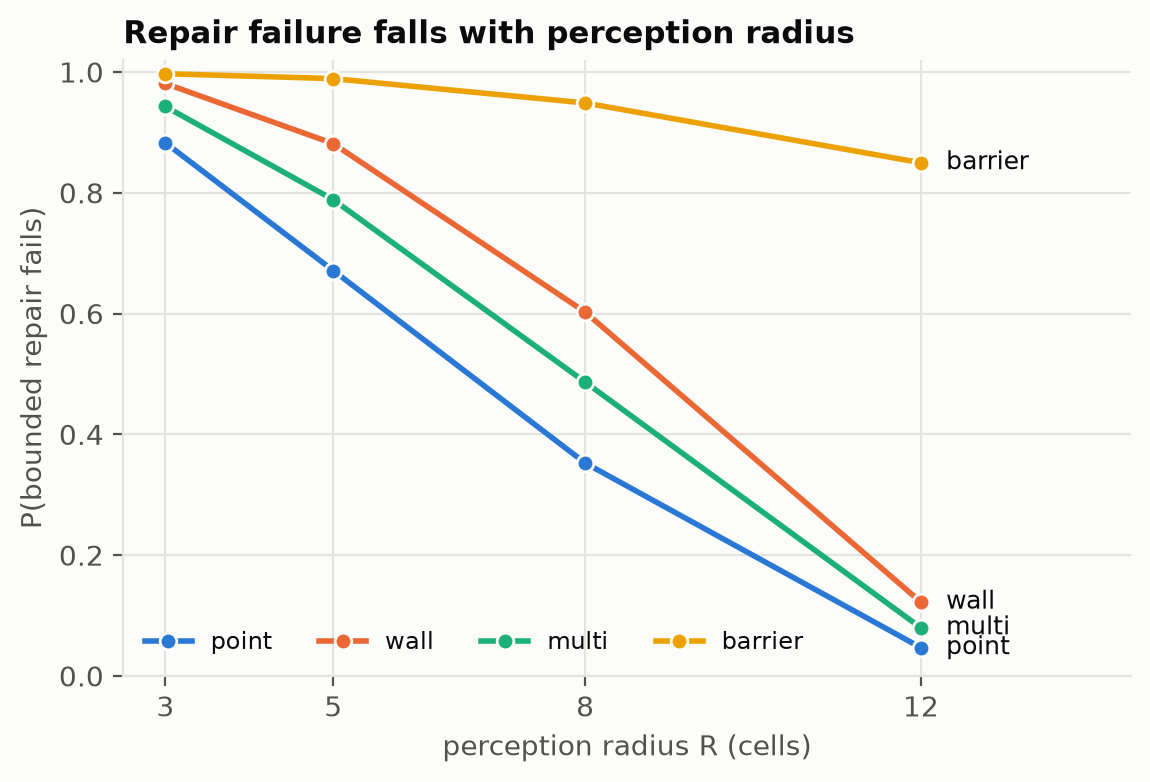
\includegraphics[width=0.62\linewidth]{figures/fig3_failure_vs_R.png}
\caption{Probability that perception-bounded repair fails, by perception radius and blockage type (held-out events).}
\label{fig:failR}
\end{figure}

\subsection{Does the break-even model predict where repair pays?}
We group events into 576 cells (map family $\times$ size $\times$ $R$ $\times$ blockage). In each cell we compare the prediction of Eq.~\eqref{eq:breakeven}, computed from the cell's measured $\pfail$, $\CL$ and $\CG$, with the measured outcome: whether the mean cost of repair-first is below that of the fallback. Against A* the model is correct in 97.6\% of cells (562/576; 96.8\% weighted by events). Against D* Lite it is correct in 90.8\% (523/576; 92.4\% weighted). Fig.~\ref{fig:breakeven} shows the cells.

Errors against D* Lite are asymmetric: 51 cells are predicted to favour repair but do not, and only 2 the other way. This is the expected direction. A D* Lite instance that is called only after failed repairs accumulates deferred updates, so its cost per call exceeds the every-event cost used in $p^\ast$.

\begin{figure}[t]
\centering
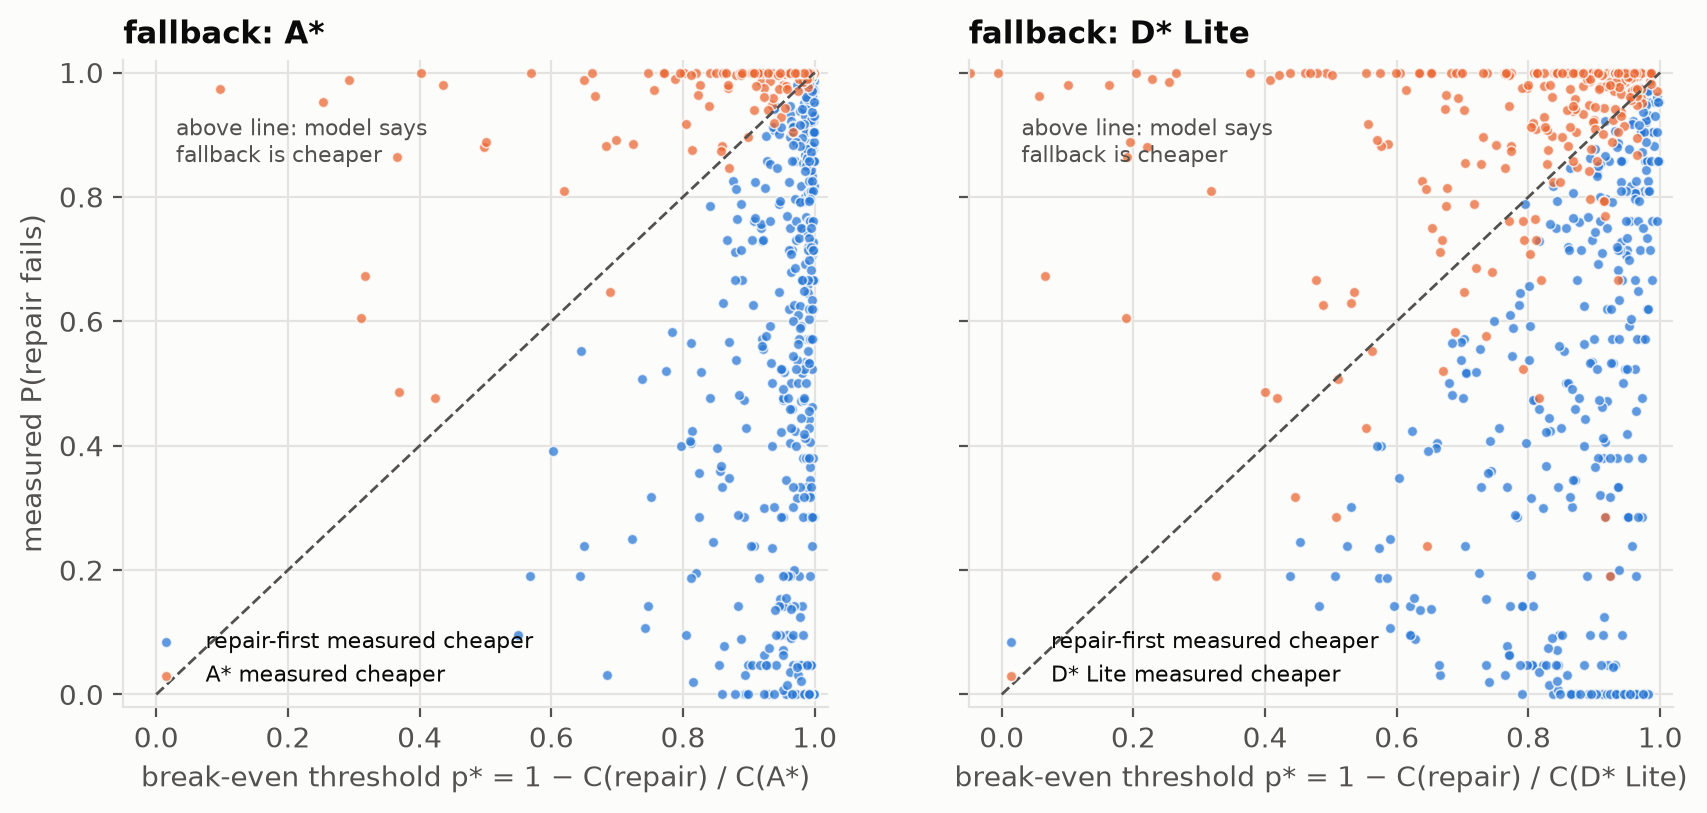
\includegraphics[width=\linewidth]{figures/fig4_break_even_validation.png}
\caption{Break-even validation over 576 cells. Each point is a cell; the dashed line is $\pfail=p^\ast$. The model predicts repair-first to be cheaper below the line. Colour shows the measured winner.}
\label{fig:breakeven}
\end{figure}

\subsection{Where does repair pay off?}
Fig.~\ref{fig:phase} shows the ratio of the cost of ``bounded repair$\to$D* Lite'' to that of D* Lite alone. Repair pays off for point, wall and multi blockages once the perception radius is large, saving up to 62\% with point blockages on $200\times200$ maps at $R=12$. At small radii the two are close, because repair fails almost always but fails cheaply. Barriers make repair a net loss everywhere, by up to 80\% on small maps with large windows, where a failed bounded search explores the whole window. Aggregated by single factors, repair-first beats D* Lite on average for $R\ge 8$ and for maps of size $\ge150$, but not for barriers or for $R\le5$.

\begin{figure}[t]
\centering
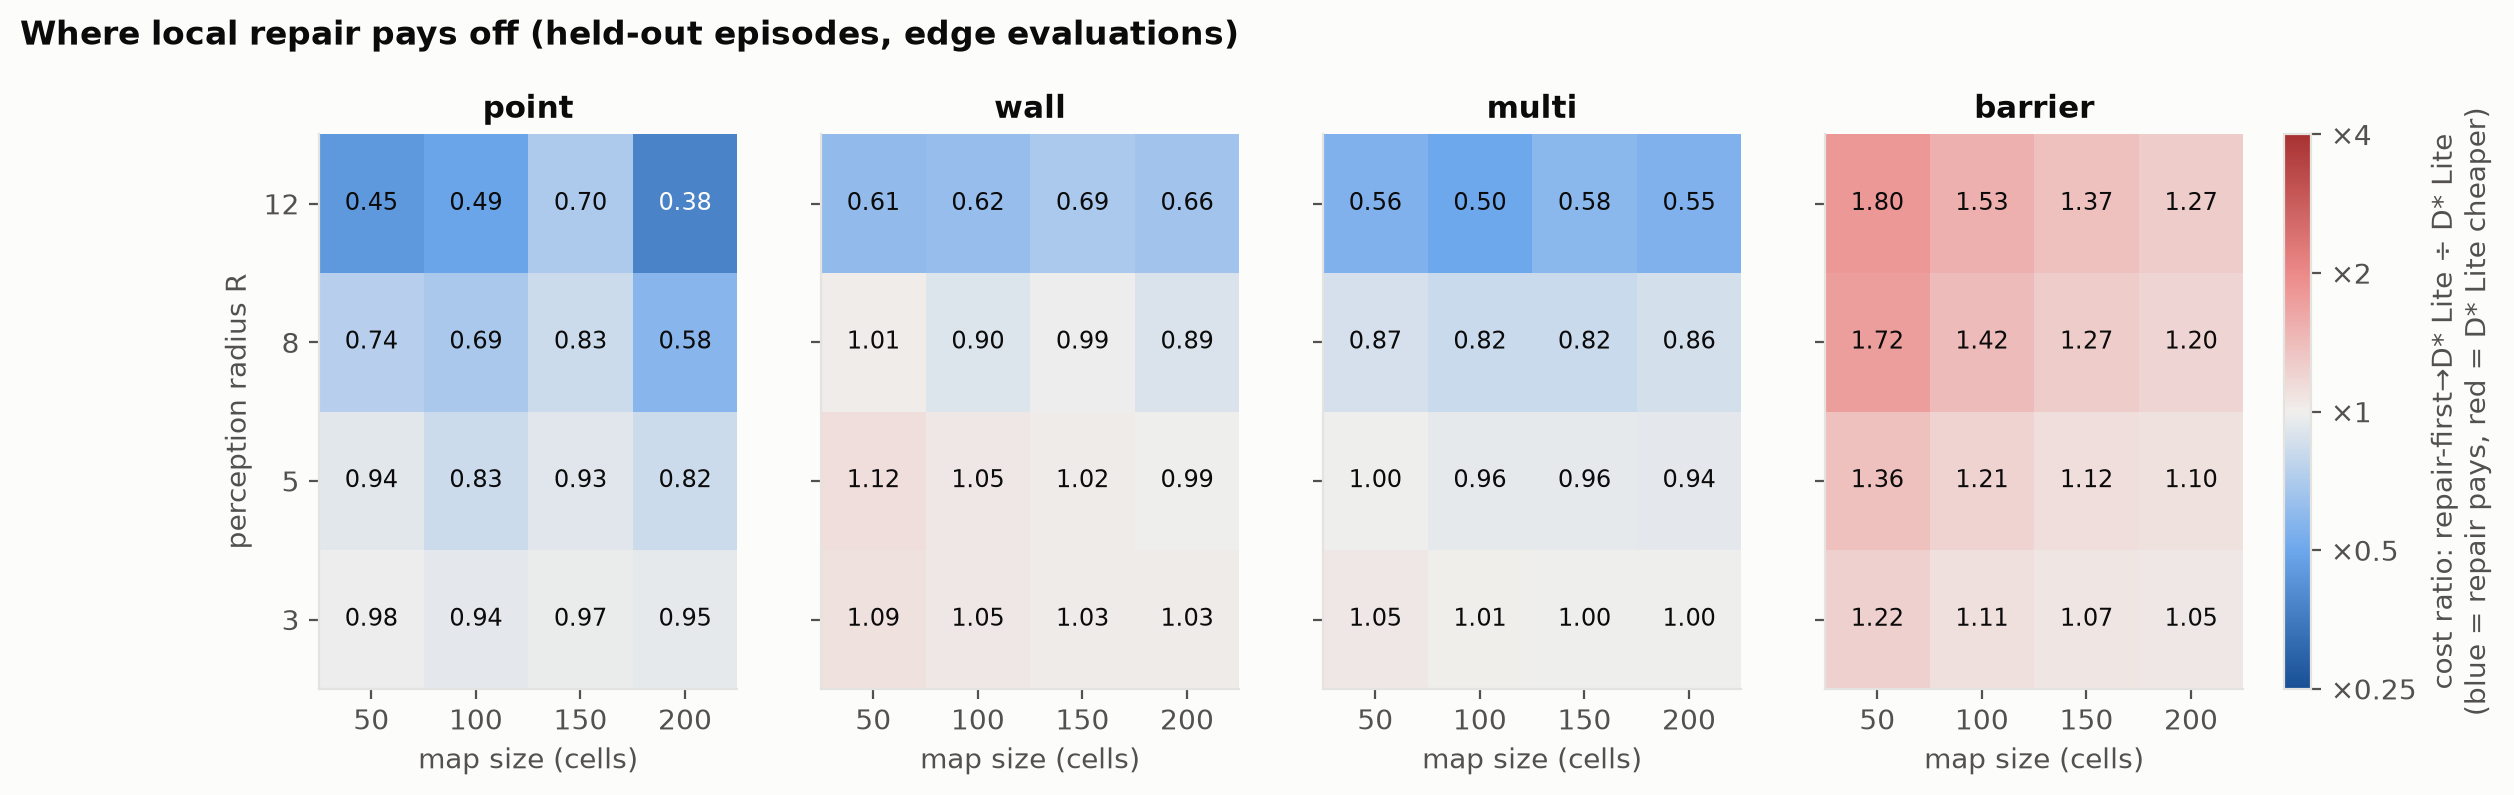
\includegraphics[width=\linewidth]{figures/fig1_phase_diagram.png}
\caption{Phase diagram: cost of bounded repair followed by D* Lite, relative to D* Lite at every event (held-out episodes). Blue cells: repair pays off; red cells: D* Lite is cheaper.}
\label{fig:phase}
\end{figure}

\subsection{Decision policies}
Table~\ref{tab:main} and Fig.~\ref{fig:policies} summarise the policies. Incremental search is essential: A* costs 5.24 times D* Lite. With bounded repair, always repairing first is 6.6\% \emph{more} expensive than D* Lite alone. The composite risk gate is indistinguishable from always repairing. It triggered on only 0.46\% of events and changed the outcome in 0.1\% of episodes (Holm-adjusted $p=0.053$). An oracle that skips doomed repairs would reach 0.877.

The learned predictor reaches 0.935 with the tuned threshold and 0.940 with the analytic break-even rule, recovering about half of the oracle gap ($(1-0.935)/(1-0.877)\approx 53\%$). Unbounded repair followed by D* Lite costs 0.651 of D* Lite's work and equals its own oracle. Its failures are all of the free kind (no splice end in the window; mean cost 0 edge evaluations), so by Sec.~\ref{sec:model} no decision model can improve on it. It is cheaper than D* Lite in 68.6\% of episodes and equal in 25.7\%, with a rank-biserial correlation of $-0.86$.

\begin{table}[t]
\centering\small
\caption{Total work (edge evaluations) relative to D* Lite at every event, held-out split ($n=\num{17472}$ episodes). CIs: cluster bootstrap over episodes. Test: Wilcoxon signed-rank on per-episode costs, Holm-adjusted; $r_{rb}$: rank-biserial correlation (negative: policy cheaper).}
\label{tab:main}
\begin{tabular}{@{}lcccc@{}}
\toprule
Policy & Ratio & 95\% CI & vs. & $r_{rb}$ ($p_{\text{Holm}}$) \\
\midrule
A* every event & 5.237 & [5.074, 5.407] & D* Lite & $+0.92$ ($<10^{-4}$) \\
D* Lite every event & 1.000 & -- & -- & -- \\
Repair (bounded)$\to$D* Lite & 1.066 & [1.054, 1.078] & D* Lite & $-0.08$ ($<10^{-4}$) \\
Risk gate$\to$D* Lite & 1.066 & [1.054, 1.078] & Repair$\to$D* & $-0.48$ (0.053) \\
Predictor, analytic$\to$D* Lite & 0.940 & [0.936, 0.944] & D* Lite & $-0.53$ ($<10^{-4}$) \\
Predictor, tuned$\to$D* Lite & 0.935 & [0.931, 0.939] & D* Lite & $-0.61$ ($<10^{-4}$) \\
Oracle, bounded repair & 0.877 & [0.870, 0.882] & -- & -- \\
\textbf{Unbounded repair$\to$D* Lite} & \textbf{0.651} & [0.639, 0.663] & D* Lite & $-0.86$ ($<10^{-4}$) \\
Oracle, unbounded repair & 0.651 & [0.639, 0.663] & -- & -- \\
\midrule
Repair (bounded)$\to$A* & 4.361 & [4.208, 4.516] & & \\
Unbounded repair$\to$A* & 2.242 & [2.156, 2.331] & & \\
\bottomrule
\end{tabular}
\\[2pt]{\footnotesize The A*-vs.-D* Lite row reports the test with A* as the reference policy; the sign convention is flipped for readability.}
\end{table}

\begin{figure}[t]
\centering
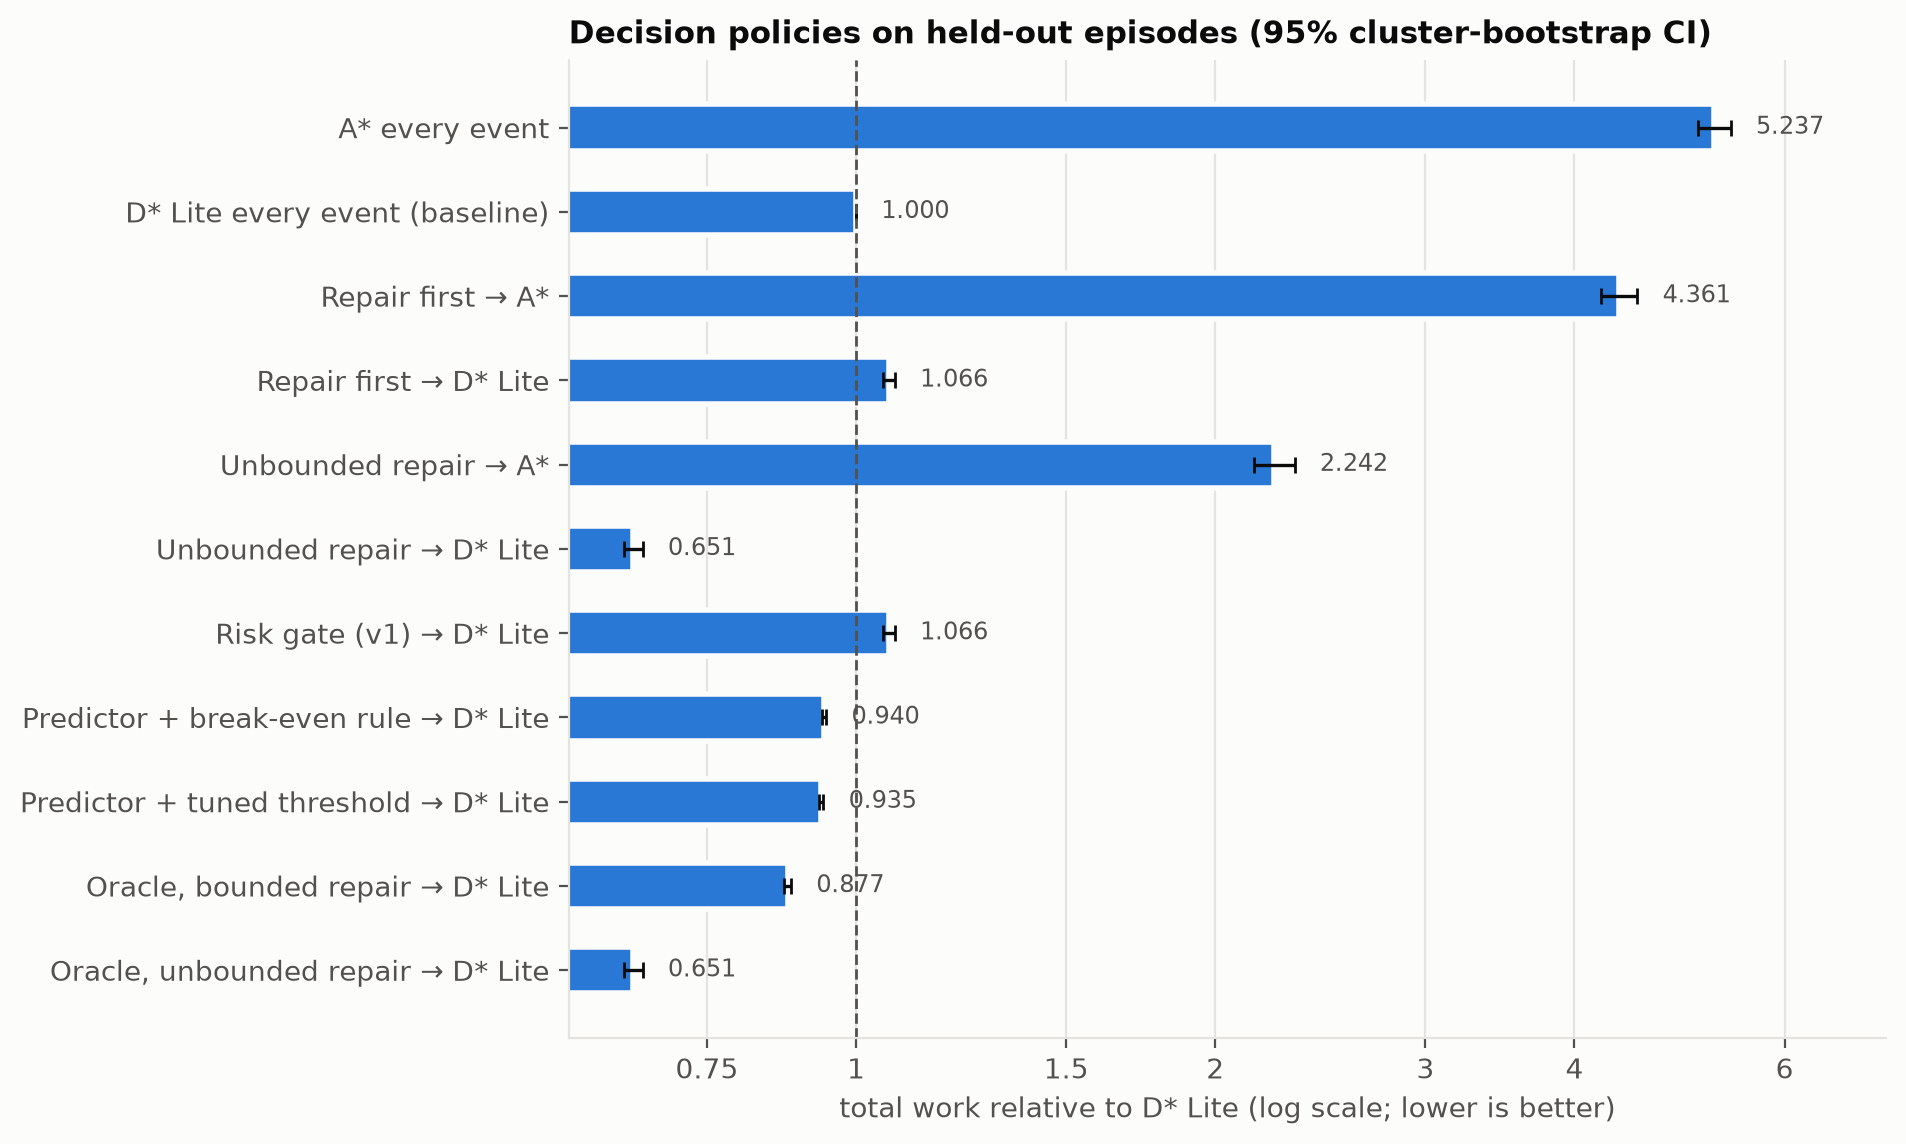
\includegraphics[width=0.85\linewidth]{figures/fig2_policy_costs.png}
\caption{Total work of each policy relative to D* Lite (log scale), with 95\% cluster-bootstrap confidence intervals.}
\label{fig:policies}
\end{figure}

\subsection{Predicting repair failure}
On held-out events the learned predictor achieves an AUC of 0.948 and a Brier score of 0.064, against a base failure rate of 79.7\%. The composite risk score achieves 0.458, which is below chance (Fig.~\ref{fig:roc}). Its components measure how much of the path is blocked and how dense new obstacles are, not whether a detour fits within the perception window, which is what decides bounded-repair success. Evaluating the predictor costs a median of 0.88\,ms per event in our Python implementation. This decision overhead is not included in the edge-evaluation metric.

\begin{figure}[t]
\centering
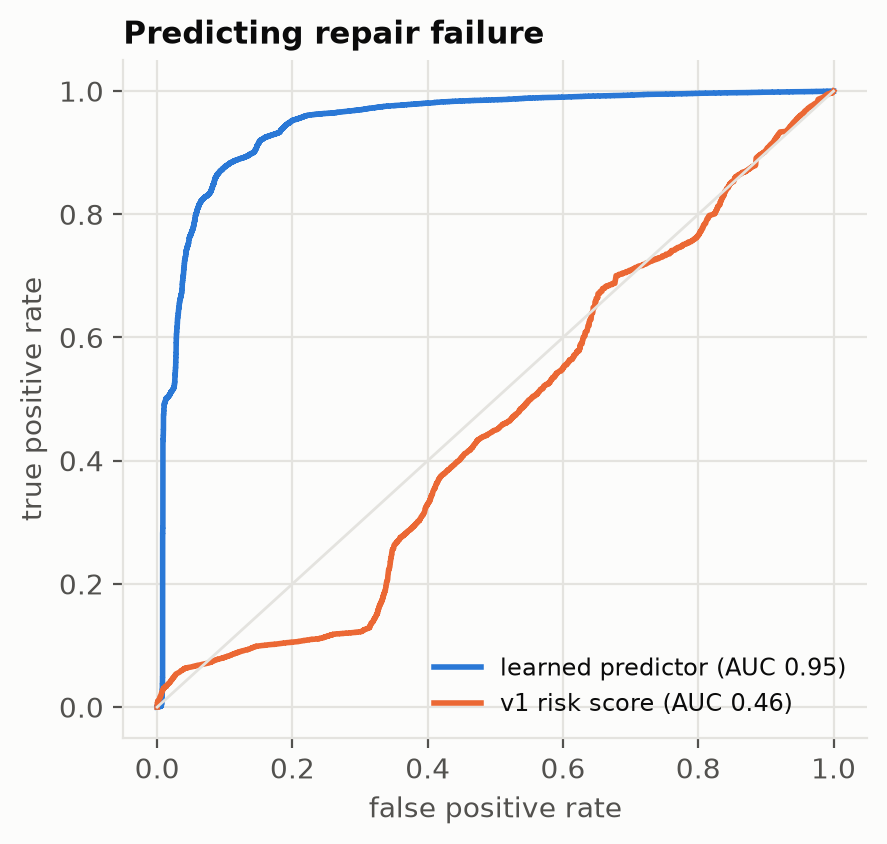
\includegraphics[width=0.45\linewidth]{figures/fig5_roc.png}
\caption{ROC curves for predicting bounded-repair failure on held-out events.}
\label{fig:roc}
\end{figure}

\subsection{Path quality, run time and generalisation}
Successful repairs lengthen the remaining path. Unbounded repair adds 7.2\% on average, 2.8\% at the median and less than 19.3\% in 90\% of cases. Bounded repair adds 6.6\% on average and 3.5\% at the median. Median wall-clock times per event were 0.37\,ms (unbounded repair), 0.52\,ms (bounded repair), 6.36\,ms (D* Lite) and 14.16\,ms (A*). Unbounded repair$\to$D* Lite is cheaper than D* Lite on every one of the nine map families (Fig.~\ref{fig:families}). The ratio ranges from 0.30 on \texttt{maze4} to 0.81 on \texttt{room8}.

\begin{figure}[t]
\centering
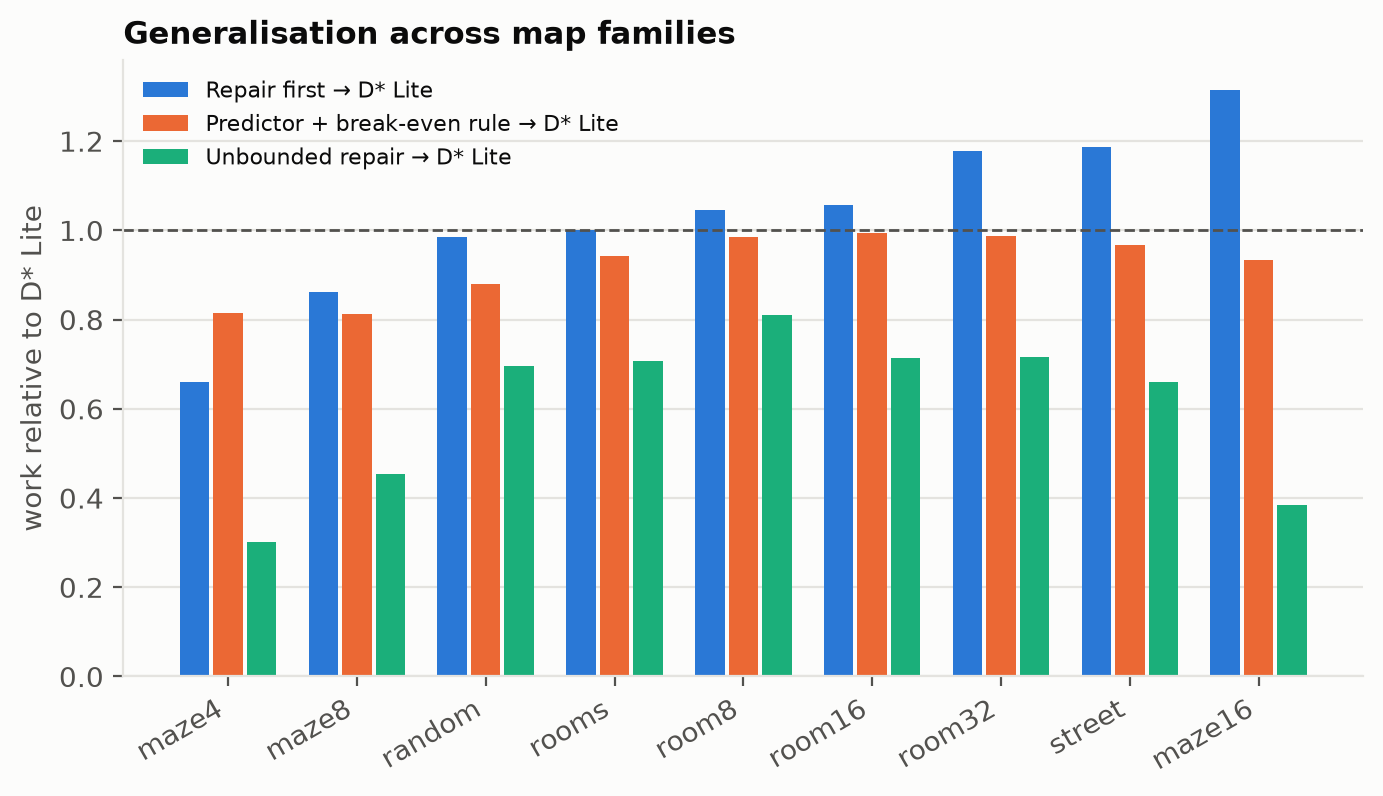
\includegraphics[width=0.8\linewidth]{figures/fig6_map_families.png}
\caption{Work relative to D* Lite per map family (held-out episodes).}
\label{fig:families}
\end{figure}

%=====================================================================
\section{Discussion}\label{sec:discussion}
%=====================================================================
\textbf{Design rules.} The results suggest three practical rules. (1)~Use an incremental planner as the fallback; repair does not compensate for replanning from scratch. (2)~Make repair failure cheap to detect. Checking that a splice end exists inside the window costs almost nothing and removes the need for any decision model: with free failure detection, always trying repair is optimal (Sec.~\ref{sec:model}) and saved 35\% of D* Lite's work here. (3)~If repair must be bounded, for example to cap worst-case latency, then whether to attempt it matters. A failure predictor with cheap, window-geometry features helps, and Eq.~\eqref{eq:breakeven} gives a principled threshold. Hand-crafted risk composites should be validated against an oracle before use; ours was uninformative.

\textbf{Why the perception radius matters.} Repair is anchored to what the robot can see: both splice points must lie in the window. Small windows make repair fail for geometric reasons that are independent of the planner, which is why $R$ is the strongest driver of failure. Sensor range, often treated as a perception parameter, is thus also a planning parameter.

\textbf{Limitations.} The study uses 2-D grids with an initially known map, discrete blockages and no sensing or actuation noise. Moving obstacles are not modelled. Costs are counted in edge evaluations of Python implementations; absolute timings would differ in optimized C++, although the counts would not. The neutral executor follows optimal paths; a robot that executes repaired paths would meet a different sequence of events, so its path-length effects compound over an episode. The analysis isolates the per-event decision. The break-even model ignores the dependence of D* Lite's per-call cost on call frequency, which makes it slightly optimistic for repair. Validation in a full navigation stack such as Nav2~\cite{macenski2020nav2} with costmaps and a physics simulator is left to future work.

%=====================================================================
\section{Conclusion}
%=====================================================================
We framed the choice between local path repair and replanning as an expected-cost decision. The resulting break-even condition, $\pfail<1-\CL/\CG$, identifies the cheaper strategy in 91--98\% of 576 experimental cells. A paired evaluation over \num{17472} held-out episodes on nine map families shows that the value of repair depends strongly on the perception radius and the blockage type. Learned failure prediction recovers about half of the oracle gap for bounded repair, whereas a hand-crafted risk composite is uninformative. When repair failure is detectable for free, ``always try repair, then D* Lite'' is optimal and costs 0.65 of D* Lite's work at a median path increase of 2.8\%.

\section*{Data and Code Availability}
Code, scenario generators, raw event tables and analysis scripts are available at [repository URL / Zenodo DOI, to be added]. Moving AI maps are available from the benchmark website~\cite{sturtevant2012}.

\bibliographystyle{unsrtnat}
\bibliography{refs}

\end{document}
